\header{
    \headtitle{Étoile des neiges} \label{etoile-des-neiges}
    %
    
    \insertComment{Chanson de Franz Winkler en allemand (1930).}{}
}

\enluminure{4}{\href{https://www.youtube.com/watch?v=koQ9LpUnCs8}{D}}{ans} un coin perdu des montagnes
\\Un tout petit Savoyard
\\Chantait son amour dans le calme du soir
\\Près de sa bergère au doux regard.
\\\\Etoile des neiges, mon coeur amoureux
\\S'est pris au piège de tes grands yeux
\\Je te donne en gage cette croix d'argent
\\Et de t'aimer toute ma vie j'en fais serment.
\\\\Hélas soupirait la bergère, que répondront nos parents ?
\\Comment ferons-nous
\\Nous n'avons pas d'argent
\\Pour nous marier dès le printemps ?
\\\\Etoile des neiges, sèche tes beaux yeux
\\Le ciel protège les amoureux.
\\Je pars en voyage pour qu'à mon retour
\\A tout jamais, plus rien n'empêche notre amour.
\\\\Alors il partit vers la ville
\\Et ramoneur il se fit
\\Sur les cheminées, sous le vent et la pluie
\\Comme un petit diable noir de suie.
\\\\Etoile des neiges, sèche tes beaux yeux
\\Le ciel protège les amoureux.
\\Ne perds pas courage, il te reviendra
\\Et tu seras bientôt encore entre ses bras.
\\\\Et quand les beaux jours refleurirent
\\Il s'en revint au hameau
\\Et sa fiancée l'attendait tout là-haut
\\Parmi les clochettes des troupeaux.
\breakpage
Etoile des neiges, tes garçons d'honneur
\\Vont en cortège portant des fleurs.
\\Par un mariage, finit mon histoire
\\De la bergère et de son petit savoyard
\\
\bigskip
\begin{center}
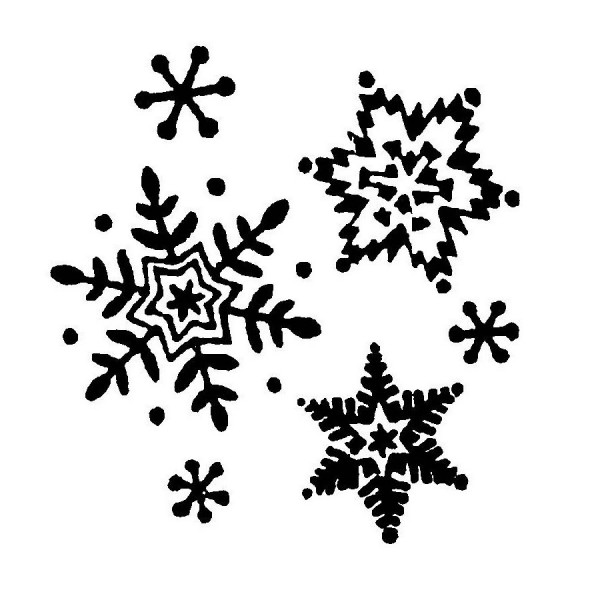
\includegraphics[width=1\textwidth]{images/flocon-de-neige.jpg}
\end{center}

\breakpage